\documentclass[11pt,a4paper,headsepline]{scrartcl}
\usepackage[utf8]{inputenc}
\usepackage[german]{babel}
\usepackage{amsmath}
\usepackage{amsfonts}
\usepackage{amssymb}
\usepackage{tikz}
\usepackage[left=2cm,right=2cm,top=2cm,bottom=2cm]{geometry}
\usepackage[utf8]{inputenc}
\usepackage{graphicx}
\usepackage{pgfplots}
\usepackage{fancyhdr}
\usepackage[scaled]{helvet}

\usetikzlibrary{calc}
\newtheorem{aufgabe}{Aufgabe}


\renewcommand*\familydefault{\sfdefault}
\renewcommand{\arraystretch}{1.1}

\title{\"Ubungen Projektmanagement}
\date{}
\makeatletter
\let\Title\@title
\let\Author\@author
\makeatother
\pagestyle{fancy}
\fancyhead[L]{Prof. Dr. Raphael Pfaff}
\fancyhead[R]{86512: Herstellung und Vermarktung}
\fancyfoot[L]{Datei: \jobname}
\fancyfoot[R]{Datum: \today \hspace{.3cm}
\begin{picture}(0,0)(0,0)\put(.5,0){
\includegraphics[height=4cm]{fh_logo}}\end{picture}}

\begin{document}
\vspace{-1cm}
\maketitle
\thispagestyle{fancy}
\pagestyle{fancy}
\vspace{-2cm}

\section*{Ausgangslage}
Der Studiengang Schienenfahrzeugtechnik hat vom Rektorat eine F\"orderung zum Bau einer Parkbahn-Lokomotive zur Teilnahme an der Railway Challenge bekommen. Das Projekt wird von Studierenden verschiedener Module bearbeitet werden.
\begin{center}
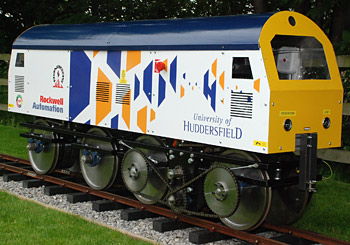
\includegraphics[width = 0.6\textwidth]{Lok}
\end{center}

\begin{aufgabe}[Projektorganisation] 
Wie beantwortet Ihr (das Projektteam) folgende Fragen:
\begin{itemize}
\item Wie binden wir Projekte in unseren Studiengang und unseren Studienalltag ein?
\item Welche standardisierten Vorgehensmodelle wenden wir an?
\item Wie stellen wir sicher, dass alle Informationen zur richtigen Zeit verf\"ugbar sind?
\item Welche Dokumente/Dokumentenarten werden eingesetzt? Wie werden sie verwaltet?
\item Gibt es Verhaltensregeln f\"ur das Projektteam?
\item Wie sichern wir die Qualit\"at der Projektbearbeitung?
\end{itemize}
Macht Vorschl\"age f\"ur das Projektteam.
\end{aufgabe}

\begin{aufgabe}[Projektorganisation] 
Welche Aufbau- und Projektorganisation erscheint Euch sinnvoll? Welche Nachteile bietet Eure Wahl?
\end{aufgabe}

\begin{aufgabe}[Projektablauf] 
L\"asst sich Euer Projekt im V-Modell abbilden? Welche Phasen sind bereits terminiert?
\end{aufgabe}

\begin{aufgabe}[Meilensteine] 
Welche Meilensteine sollten wir nutzen? Welche Anforderungen sollten wir stellen?
\end{aufgabe}

\end{document}